\section{Background}\label{sc:background}
\subsection{Rewriting Logic}

\subsubsection{Model checking?}
% Model checking \cite{clarke99,baier_principles_2008} is a technique for automated verification of complex
% reactive systems such as hardware components, embedded controllers, and network
% protocols. The technique works by expressing the specification of a system using logical formulas.


\subsection{Co-simulation}
Co-simulation is a technique enabling the global simulation of a system consisting of multiple black-box SUs. 
An SU has a dedicated solver calculating the behavior trace of the dynamical system it represents. 
A dynamical system is a function from time and space into some often multi-dimensional and continuous space. Examples include population growth, water flow, and pendulums. 
Interaction of the system with the external environment happens through inputs and outputs~\cite{Gomes2019a,Kubler2000}.

\subsection{Simulation Units}
SUs can be coupled through their inputs and outputs, indicating that the state of one SU is reliant on the state of another SU at all times - known as a coupling restriction. However, in practice, the coupling restrictions can only be satisfied at specific points in time, referred to as communication points. Furthermore, each SU makes assumptions about the evolution of the input values between the communication points, which can cause accumulable errors in the co-simulation~\cite{Arnold2014}. 

A scenario is simulated using an orchestrator - an algorithm - that computes the behavior trace of all SUs trying to satisfy their coupling restrictions by exchanging values. 
The orchestrator's goal is to find the communication points that minimize the co-simulation error and ensure that the SUs move in lockstep. 
Studies \cite{Gomes2019,Oakes2021,Gomes2018f,Schweizer2015c,Gomes2018a} have shown that optimal communication points depend on the implementation of the SUs.

\begin{definition}[Simulation Unit]\label{def:fmu}
  An SU with identifier $c$ is represented by the tuple
  $$\tuple{\stateset{c}, \inputs{c}, \outputs{c}, \fset{c}, \fget{c}, \fdoStep{c}},$$
  where:
  \begin{compactitem}
    \item $\stateset{c}$ represents the state space.
    \item $\inputs{c}$ and $\outputs{c}$ the set of input and output variables, respectively. 
    \item $\fset{c} : \stateset{c} \times \inputs{c} \times \valuesExchanged \to \stateset{c}$ and $\fget{c}: \stateset{c} \times \outputs{c} \to \valuesExchanged$ are functions to set the inputs and get the outputs, respectively (we abstract the set of values exchanged between input/output variables as $\valuesExchanged$. The type of this set is the tuple $\tuple{t, \values}$, where $\values$ denotes the value obtained at a given output port and $t: \timebase$ denotes the timestamp of $c$ when the value was obtained by an action respecting the contracts).
    \item $\fdoStep{c}: \stateset{c} \times \stepbase \to \stateset{c} \times \stepbase $ is a function that instructs the SU to compute its state after a given time duration. If an SU is in state $\stateafter{c}{t}$ at time $t$, $(\stateafter{c}{t+h}, h) = \fdoStep{c}(\stateafter{c}{t}, H)$ approximates the state $\stateafter{c}{t+h}$ of the corresponding model at time $t+h$, where $h \leq H$. 
  \end{compactitem}
\end{definition}
\vspace{-0.5em}
\Cref{def:fmu} is inspired by \cite{Broman2013,Gomes2019c,thrane2021} and represents a symbolic version of an SU. 
The state of SU $A$ at time $t$ is denoted $\stateafter{A}{t}$.
We assume the last value set on an input/output port can be inspected, for example, the value of input $\inputvar{x}$ could be $\inputvar{x} = \tuple{t, v_x}$, where $t$ is the timestamp when the value $v_x$ set on $\inputvar{x}$ was obtained.
The function $\fdoStep{c}$ returns a step size because some SUs implement error estimation and may conclude that taking a step size of $H$ will result in an intolerable error meaning the SU takes a smaller step than planned.

\begin{definition}[Scenario]\label{def:cosim_scenario}
  A scenario is a structure $\tuple{\fmus, \coupling, \mayReject, \allfeedthroughs, \allreactivity, \alldelayed}$ where each identifier $c \in \fmus$ is associated with an SU, as defined in \cref{def:fmu}, and $\coupling(u)=y$ means that the output $y$ is connected to input $u$.
  Let $\allinputs = \bigcup_{c \in \fmus} \inputs{c}$ and $\alloutputs = \bigcup_{c \in \fmus} \outputs{c}$, then $\coupling : \allinputs \to \alloutputs$. 
  $\mayReject \subseteq \fmus$ denotes the SUs that implement error estimation. 
  The set of reactive components,
  $\allreactivity = \bigcup_{c \in \fmus} \reactivity{c}$, where $\reactivity{c}(\inputvar{c}) = \true$ means the function $\fdoStep{c}$ assumes that the input $\inputvar{c}$ comes from an SU that has advanced forward relative to SU $c$.  
The set of delayed components,
  $\alldelayed = \bigcup_{c \in \fmus} \neg \reactivity{c}$, where $\reactivity{c}(\inputvar{c}) = \false$ means the function $\fdoStep{c}$ assumes that the input $\inputvar{c}$ comes from an SU that is at the same time as SU $c$. 
 Finally, the set of feed-through components, $\allfeedthroughs = \bigcup_{c \in \fmus} \feedthrough{c}$, where the input $\inputvar{c} \in \inputs{c}$ feeds through to output $\outputvar{c} \in \outputs{c}$, that is, $(\inputvar{c},\outputvar{c}) \in \feedthrough{c}$, when there exists $v_1, v_2 \in \valuesExchanged$ and $\state{c} \in \stateset{c}$, such that
  $\fget{c} (\fset{c}(\state{c}, \inputvar{c}, v_1), \outputvar{c}) \neq \fget{c} (\fset{c}(\state{c}, \inputvar{c}, v_2), \outputvar{c}).$
\end{definition}  

The syntax in \cref{fig:simpleexample} is used to graphically present co-simulation scenarios.
A scenario can contain cyclic dependency between different ports, these are denoted algebraic loops.
The algebraic loops are a consequence of the couplings of the SUs and feedthrough. 
An example of an algebraic loop is depicted in \cref{fig:algebraic_example}.
The port variables in that scenario form a cyclic dependency, requiring that all their values are being set at the same time. 
The set of port variables involved in algebraic loops are the port variables of the non-trivial SCCs in the step operation graph, constructed based on Definition 15 in \cite{Gomes2019c}.
The set $\algebraic{S}$ denotes such variables in scenario $S$:
%\vspace{-0.5em}
\begin{align*}
  \algebraic{S} \triangleq \{s \mid \text{for each\ } s \in \mathit{SCCs} \land s \in \allinputs \cup \alloutputs\}, \\
  \text{ where } \mathit{SCCs}: \text{ is the flatten set of all nontrivial SCCs in S}.
\end{align*}
\vspace{-0.5em}

\begin{wrapfigure}{I}{0.5\textwidth}
  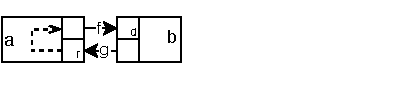
\includegraphics[width=0.5\textwidth]{images/simple_example.pdf}
  \caption{A simple co-simulation scenario ($S1$).}
  \label{fig:simpleexample}  
\end{wrapfigure}

The input variables involved in an algebraic loop in the scenario $S$ are:
\begin{align}
  \inputs{\algebraic{S}} \triangleq \algebraic{S} \cap \allinputs
\end{align}

A scenario is either simple or complex.
\begin{definition}\label{def:simpleScenario}
  A scenario $S$ is simple if $\mayReject = \emptyset \land \algebraic{S} = \emptyset$.
\end{definition}

A scenario is complex if it is not simple. Using \cref{def:simpleScenario} we conclude that the scenario ($S1$) in \cref{fig:simpleexample} is simple because $\algebraic{S1}=\emptyset$ and none of the SUs implement error estimation ($\mayReject_{S1}=\emptyset$). The scenario ($S2$) in \cref{fig:algebraic_example} is complex since $\algebraic{S2}=\{\inputvar{f}, \inputvar{g}, \outputvar{f}, \outputvar{g}\}$ meaning that all variables are a part of a cyclic dependency that should be solved using a fixed point.
The scenario ($S3$) in \cref{fig:step_finding_scenario} is also complex because SU $C$ implements error estimation ($\mayReject_{S2}=\{C\}$) and therefore can perform step rejection. Step rejection requires special attention since the orchestrator should backtrack the simulation and restart the simulation with a smaller step in case of a step rejection.

The reason for distinguishing between simple and complex scenarios is that the simulation strategy depends on the scenario type. This is treated in more detail later in the paper.
Next, we give a brief presentation of the contracts from \cite{Gomes2019a} before describing how they can be used to verify a co-simulation algorithm.

\begin{figure}[htb]
  \begin{subfigure}{0.48\textwidth}
    \centering
    \centering
    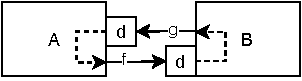
\includegraphics[width=0.9\textwidth]{images/scenario_algebraic.pdf}
    \caption{Scenario $S2$ with an algebraic loop.}
    \label{fig:algebraic_example}
  \end{subfigure}
  \begin{subfigure}{.48\textwidth}
    \centering
    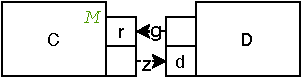
\includegraphics[width=0.95\textwidth]{images/step_negotiation_scenario.pdf}
    \caption{Scenario $S3$ needs step negotiation.}
    \label{fig:step_finding_scenario}
    \end{subfigure} 
    \caption{Complex co-simulation scenarios.}
    \vspace{-2em}

  \end{figure}

The contracts are described as preconditions of the SU-actions $\fget{}$, $\fset{}$ and $\fdoStep{}$.
It should be pointed out that each input and output has a timestamp referring to when it was last successfully activated by an action. 
%\vspace{-0.8em}
\begin{definition}[Get Action]\label{def:getout}  
  The precondition of $\fget{c}(\stateafter{c}{t}, \outputvar{c})$ is: \\
  $\forall (\inputvar{\dontcare}, \outputvar{c}) \in \feedthrough{c} \implies \inputvar{\dontcare} = \tuple{t_h, \dontcare} \land t_h = t$.\\
  Informally saying that all inputs that feeds through to $\outputvar{c}$ should be set.
  This criterion is denoted as the predicate: $\fpreget{c}: \stateset{c} \times \outputs{c} \to \mathbb{B}$.
\end{definition}
%\vspace{-1em}
\begin{definition}[Set Action]\label{def:setin}
  The precondition of $\fset{c}(\stateafter{c}{t}, \inputvar{c}, \inputV)$ depends on the contract of the input:
  \begin{compactitem}
    \item If $\inputvar{c} \in \allreactivity$ then the operation is valid if $\inputV= \tuple{t_h,\dontcare}, \textrm{ where } t_h = t+H$
    \item If $\inputvar{c} \in \alldelayed$ then the operation is valid if $\inputV= \tuple{t_h,\dontcare}, \textrm{ where } t_h = t$.
  \end{compactitem} 
  This informally says that the value set on $\inputvar{c}$ should be obtained at a meaningful point in time dictated by the input contract.
  We denote this as the predicate: $\fpreset{c}: \stateset{c} \times \inputs{c} \times \valuesExchanged  \to \mathbb{B}$.
  \end{definition}

  The criterion on a set-action will first have an effect when the SU is stepped. However, we found that it was easier to catch and correct an incorrect algorithm by moving this criterion to the set-action. 
  
  %\vspace{-1em}
  \begin{definition}[Step Computation]\label{def:step}
  The precondition of $\fdoStep{c}(\stateafter{c}{t}, H)$ is satisfied if all the following conditions are fulfilled:
  \begin{compactitem}
    \item $\forall \inputvar{c} \in \inputs{c} \ldotp \inputvar{c} \in \alldelayed \implies \inputvar{c} = \tuple{t_h,\dontcare} \land t_h = t$. 
    \item  $\forall \inputvar{c} \in \inputs{c} \ldotp \inputvar{c} \in \allreactivity \implies \inputvar{c} = \tuple{t_h,\dontcare} \land t_h = t + H$.
    %\item $\fdoStep{c}(\stateafter{c}{t},H)=(\dontcare,H)$
  \end{compactitem}
  Informally, this is that all inputs should set with a new value since the last time the SU was stepped.
  This is denoted as the predicate: $\fpredoStep{c}: \stateset{c} \times \stepbase \to \mathbb{B}$.
  \end{definition}
%\vspace*{-1.4em}
\begin{definition}[Preconditions of a Scenario]\label{def:precondition}
  The set of all preconditions $\precondition$ of a scenario is the union of the preconditions for each SU $c \in \fmus$:
  \begin{align}
    \precondition = \bigcup_{c \in \fmus} \set{\bigcup_{i \in \inputs{C}}\fpreset{c}(\dontcare, \inputvar{i}, \dontcare), \bigcup_{i \in \outputs{C}}\fpreget{c}(\dontcare, \outputvar{i}), \fpredoStep{c}}
  \end{align}
\end{definition}

The SU inspired by the FMI-standard~\cite{FMI2014} is a state-machine, the  SU as a state-machine.
The formalization in Maude enforces them, but they are treated in this paper.

\subsection{Co-simulation algorithms}\label{sc:cosimalgo}
A scenario is , as described, simulated by a co-simulation algorithm that consists of state-changing functions, an initialization procedure, and a co-simulation step. 
%This work concentrates on the co-simulation step, which we refer to as the algorithm throughout the paper. The other aspects of a co-simulation algorithm can trivially be derived from the method.  

The purpose of the co-simulation step is to advance all SUs $\fmus$, and all inputs and outputs $(\allinputs \cup \alloutputs)$, from the initial times $t$ to a future time $t+H, \textrm{ where } H > 0$. 
We use function $\ftime: \stateset{C} \to \timebase$ to obtain the current timestamp of an SU.
This makes it possible to define the Hoare-triple of the co-simulation step $P$:
\begin{align*}
  Hoare(P) \,\triangleq\, &\{\forall v \in \allinputs \cup \alloutputs \ldotp v = \tuple{t, \dontcare} \land \forall c \in \fmus \ldotp \ftime(\stateafter{c}{t}) = t\} \qquad  P \\
  & \qquad \{\forall v \in \allinputs \cup \alloutputs \ldotp v = \tuple{t+H, \dontcare} \land \forall c \in \fmus \ldotp \ftime(\stateafter{c}{t+H}) = t+H \}
\end{align*}

A co-simulation step $P$  is a sequence of instructions using the SU's functions $\fset{c},\fget{c}$, and $\fdoStep{c}$. 
Each index $i$ of the sequence $P[i]$ represents an action in the algorithm, for example, if $P$ is the co-simulation step in \cref{alg:algorithm_1} $P[0] = \fdoStep{A}(\stateafter{A}{0}, \dontcare)$. \Cref{fig:algorithms} shows three different co-simulation steps of the scenario in \cref{fig:simpleexample}. 
\vspace{-1em}
\begin{figure}[htb]
  \centering
  \begin{minipage}[t]{.325\textwidth}
    \begin{algorithm}[H]
      \caption{}
      \label{alg:algorithm_1}
      \begin{algorithmic}[1]
        \scriptsize
        \State $(\stateafter{A}{H},H) \gets \fdoStep{A}(\stateafter{A}{0}, H)$
        \State $(\stateafter{B}{H},H) \gets \fdoStep{B}(\stateafter{B}{0}, H)$
        \State $f_{v} \gets \fget{A}(\stateafter{A}{H}, \outputvar{f})$
        \State $g_{v} \gets \fget{B}(\stateafter{B}{H}, \outputvar{g})$
        \State $\stateafter{B}{H} \gets \fset{B}(\stateafter{B}{s}, \inputvar{f}, f_{v})$
        \State $\stateafter{A}{H} \gets \fset{A}(\stateafter{A}{H},\inputvar{g},g_{v})$
      \end{algorithmic}
    \end{algorithm}
  \end{minipage}
  \begin{minipage}[t]{0.325\textwidth}
    \begin{algorithm}[H]
      \caption{}
      \label{alg:algorithm_2}
      \begin{algorithmic}[1]
        \scriptsize
        \State $(\stateafter{B}{H},H) \gets \fdoStep{B}(\stateafter{B}{0}, H)$
        \State $(\stateafter{A}{H},H) \gets \fdoStep{A}(\stateafter{A}{0}, H)$
        \State $g_v \gets \fget{B}(\stateafter{B}{H}, \outputvar{g})$
        \State $\stateafter{A}{H} \gets \fset{A}(\stateafter{A}{H}, \inputvar{g}, g_v)$
        \State $f_v \gets \fget{A}(\stateafter{A}{H}, \outputvar{f})$
        \State $\stateafter{B}{H} \gets \fset{B}(\stateafter{B}{H}, \inputvar{f}, f_v)$
      \end{algorithmic}
    \end{algorithm}
  \end{minipage}
  \begin{minipage}[t]{0.325\textwidth}
    \begin{algorithm}[H]
      \caption{}
      \label{alg:algorithm_3}
      \begin{algorithmic}[1]
        \scriptsize
        \State $(\stateafter{B}{H},H) \gets \fdoStep{B}(\stateafter{B}{0}, H)$
        \State $g_v \gets \fget{B}(\stateafter{B}{H}, \outputvar{g})$
        \State $\stateafter{A}{0} \gets \fset{A}(\stateafter{A}{0}, \inputvar{g}, g_v)$
        \State $f_v \gets \fget{A}(\stateafter{A}{0}, \outputvar{f})$
        \State $\stateafter{B}{H} \gets \fset{B}(\stateafter{B}{H}, \inputvar{f}, f_v)$
        \State $(\stateafter{A}{H},H) \gets \fdoStep{A}(\stateafter{A}{0}, H)$
      \end{algorithmic}
    \end{algorithm}
    \vspace{4pt}
  \end{minipage}
  \vspace{-2em}
  \caption{Three algorithms conforming to the FMI Standard (version 2.0) of the scenario in \cref{fig:simpleexample}.}
  \label{fig:algorithms}
%  \vspace{-1em}
\end{figure}

Although the three algorithms in \cref{fig:algorithms} consist of the same actions, they are not equivalent, and simulating with one algorithm instead of one of the others could drastically change the co-simulation result as shown in \cite{Gomes2019c}. 
They showed that by obeying the contracts, the scenario will be simulated correctly. We assume that the contracts in the scenario are constant through the simulation, which is the case for most commercially used SUs.
At the end of \cref{sec:correctcosim}, we show which of these algorithms is correct.

A co-simulation step $P$ is executed using a configuration $c$. The configuration $c \triangleq \tuple{H, guess}$ consists of the parameters of the co-simulation step $P$.  $H \in \stepbase$ defines the step size, and $guess : \inputs{algebraic} \to \valuesExchanged$ is a total function linking all inputs in $\inputs{algebraic}$ to a guess that tries to satisfy the algebraic loops. Using the example from \cref{alg:algorithm_1}, the action at index 0 in $P$ applied with the configuration $\tuple{1,\dontcare}$ is: $P[0](c) = \fdoStep{A}(\stateafter{A}{0}, 1)$. The configuration defines the step size $(1)$ of the step-action. 

The set $\configuration$ denotes all the possible configurations of the co-simulation step for a given scenario. The execution of a co-simulation step $P$ is the execution of each action in $P$. We define such execution of $P$ using configuration $c$ as:
\vspace{-1em}
\begin{align}
  P(c) \triangleq \text{for each } i \in \dom{P} \ldotp P[i](c)
\end{align}
An execution of $P(c_j)$ yields another configuration $c_{j+1} \in \configuration$ where $P(c_j) = c_{j+1}$. The configuration $c_{j+1}: \tuple{H_1, guess_1}$ is obtained from the algorithm $P$ and configuration $c_j: \tuple{H, guess}$ by updating $H_1$ to the smallest step accepted by an SU during the execution of $P(c_j)$. And the function $guess_1$ has the same domain as $guess$, but the range is updated to the new value of the output coupled to the associated input in the domain of $guess$ after executing $P(c_j)$.
\vspace{-1em}
\begin{align}
  guess_{j+1}(u) = value(u,P(c_j)) \text{ and } H_1 = minStep(P(c_j))  
\end{align}  
The execution of a configuration $c: \tuple{H, guess}$ has converged if all SUs accept the step $H$, and all algebraic loops are stabilized (all values in the range of $guess$ are fixed-points). 
The domain of $guess$ is all the inputs in $\inputs{algebraic}$ for the scenario; this means that all configurations of the same scenario have the same domain.
\begin{definition}\label{def:convergent}
  Two configurations of the same scenario S $c_j:\tuple{H_1,guess_1} \in \configuration$ and $c_{j+1}: \tuple{H_2, guess_2} \in \configuration$ are convergent if:
  \vspace{-1em}
  \begin{align*}
    c_j \approx c_{j+1} \triangleq H_1 = H_2 \land (\forall i \in \dom{guess} \ldotp guess_1[i] \approx guess_2[i])
  \end{align*}
  Two values $v1_E: (v_1, t_1)$ and $v2_E: (v_2, t_2)$ of type $\valuesExchanged$ converge if:
  \begin{align}
    v1_E \approx v2_E \triangleq \, \mid v_1 - v_2 \mid \ \leq \epsilon \land t_1 = t_2
  \end{align}
\end{definition}

Formally an execution of a co-simulation step $P$ of a configuration $c_j$ is stable or has converged if $P(c_j) = c_{j+1} \implies c_j \approx c_{j+1}$.
% All configurations are stable for simple scenarios defined by \cref{def:simpleScenario}. 
% \begin{lemma}\label{def:simple}
%   A scenario is simple if all configurations of the algorithm $P$ converge: 
%   \begin{align*}
%     \forall c_j,c_{j+1} \in \configuration \ldotp P(c_{j}) = c_{j+1} \implies c_j \approx c_{j+1}
%   \end{align*}
% \end{lemma}

A complex scenario is a scenario where not all configurations are stable. Such a scenario can only be correctly simulated by an algorithm $P$ if a convergent configuration exists:
\vspace{-1em}
\begin{align}
  \exists c \in \configuration, \exists j \in \setnat \ldotp P(c_{j}) = c_{j+1} \implies c_{j} \approx c_{j+1}
\end{align}
Some measures should be taken to handle cases where no convergent configuration exists.

\subsection{Correct Co-simulation Algorithms}\label{sec:correctcosim}
To optimally simulate a co-simulation scenario using an algorithm $P$ requires more than a convergent configuration $c$. The algorithm $P$ should also successfully satisfy all the preconditions/contracts. To describe this, we introduce the sequence $\allcontracts$, which is a permutation of the set $\precondition$ (cf.\ \cref{def:precondition}).
The sequence $\allcontracts$ is constructed by a function $\allcontracts = \mathit{contracts(P, \precondition)}$ that for each action in $P$ finds the corresponding precondition $pre \in \precondition$ and adds it to $\allcontracts$ such that for an arbitrary index $i$ in $P$, $\allcontracts[i]$ is the precondition of the action $P[i]$.

If an action at index $i$ in $P$ satisfies its precondition $\allcontracts[i]$ using the configuration $c$, it is denoted as:
\vspace{-1em}
\begin{align}
  P[i](c) \models \allcontracts[i]
\end{align}
A co-simulation step $P$ using a configuration $c$ satisfies $\allcontracts$ if all actions satisfy its precondition. 
\vspace{-1em}
\begin{align}
  P(c) \models \allcontracts \triangleq \forall i \in \dom{P} \ldotp P[i](c) \models \allcontracts[i]
\end{align}
$P(c) \models \allcontracts$ means the algorithm respects the scenario's contracts.
Based on previous studies it is well-known that a non-convergent configuration $c$ does not respect all the contracts:
\vspace{-1em}
\begin{align}\label{eq:incorrectConf}
  c_j \not\approx c_{j+1} \implies P(c_j) \not\models \allcontracts
\end{align}
Therefore we only check the contracts of the scenario if the current configuration is convergent.
We can now describe what it means for an algorithm to be correct for a given scenario in the following Hoare triple.

\begin{definition}\label{def:correctalgo}
  An algorithm $P$ and configuration $c: \tuple{H, \dontcare}$ is correct if:
  \vspace{-0.5em}
  \begin{align*}
     P(c) \models \allcontracts \quad \land \quad
     &\{\forall v \in \allinputs \cup \alloutputs \ldotp v = \tuple{t, \dontcare} \land \forall c \in \fmus \ldotp \ftime(\stateafter{c}{t}) = t\} \quad P(c) \\
     & \{\forall v \in \allinputs \cup \alloutputs \ldotp v = \tuple{t+H, \dontcare} \land \forall c \in \fmus \ldotp \ftime(\stateafter{c}{t+H}) = t+H \}
  \end{align*}
  Meaning all preconditions are satisfied and all SUs and inputs have moved from time $t$ to time $t+H$ through the execution of $P(c)$.
\end{definition}
\vspace{-0.5em}

Using \cref{def:correctalgo} we conclude that \cref{alg:algorithm_3} is correct while the others are incorrect since they break one or more of the defined preconditions. \Cref{alg:algorithm_1,alg:algorithm_2} violate the precondition of $\fdoStep{b}$ on line 2 by stepping it without having provided SU $b$ with a value on the reactive input $f$. 
These definitions form the basis for describing the approach and implementation used to verify co-simulation algorithms in this work.